\chapter{مسائل و مشکلات Virtualbox}
\setlatintextfont{Times New Roman}
\section{نصب}
\label{vboxA}
فایل نصبی برنامه \lr{Virtualbox} را می\nf توان از سایت \lr{virtualbox.org}، متناسب با نوع سیستم عامل خود دانلود کرد. توصیه می\nf شود که \lr{Virtualbox} بر روی سیستم عامل اوبونتو نصب شود. برای نصب بر روی سیستم عامل اوبونتو، پس از دریافت فایل نصبی، از طریق خط فرمان،\ به پوشه\nf ای که فایل در آن ذخیره شده است\RTLfootnote{معمولاً پوشه\nf ی \lr{Download}}  رفته و دستور زیر را اجرا کنید:
\begin{latin}
\noindent  1. sudo dpkg -i virtualbox*
\end{latin}

روش دیگر، نصب بسته از طریق مخازن نرم\nf افزار است. ابتدا مخازن خود را با دستور شماره  \lr{2} به\nf روز کرده و سپس دستور شماره \lr{3} را اجرا کنید. در صورت موجود نبودن نرم\nf افزار \lr{Virtualbox} در مخازن و عدم نصب آن، با دستورات \lr{4} تا \lr{6}، کلید مخازن \lr{Virtualbox} و مخزن آن را به سیستم خود اضافه کرده و سپس، دستورات \lr{2} و \lr{3} را اجرا کنید. البته ممکن است به دلیل فیلترینگ و یا عدم اجازه\nf ی دسترسی کاربران ایران به مخازن  \lr{Virtualbox}، استفاده از این روش امکان\nf پذیر نباشد.
\begin{latin}
\setlength{\parindent}{0ex}
2. sudo apt-get update

3. sudo apt-get install virtualbox

4. wget -q https://www.virtualbox.org/download/oracle\_ vbox\_ 2016.asc -O- | sudo apt-key add -

5. wget -q https://www.virtualbox.org/download/oracle\_ vbox.asc -O- | sudo apt-key add - 

6. sudo sh -c 'echo "deb http://download.virtualbox.org/virtualbox/debian \$(lsb\_ release -sc) contrib" >> /etc/apt/
sources.list.d/virtualbox.list'
\end{latin}

\section{خطای اجرا کردن ماشین مجازی}
\label{vboxAA}
پس از نصب \lr{Virtualbox} و اضافه کردن ماشین مجازی موردنظر، ممکن است در هنگام اجرای ماشین مجازی با خطای \lr{Required key not available} و یا خطاهایی با این مضمون مواجه شوید. دلیل وجود این خطا، عدم اجازه\nf ی اجرای ماژول\nf های کرنل امضانشده\RTLfootnote{\lr{Unsigned Kernel Module}} توسّط کرنل\nf های اوبونتوی نسخه\nf ی \lr{4.4.0} به بعد است. این عدم اجازه، مربوط به زمانی است که \lr{boot} امن فعّال باشد. بنابراین، برای رفع این خطا دو راه وجود دارد. راه اوّل، غیرفعّال کردن \lr{boot} امن سیستم عامل است. راه دوّم، امضاکردن این ماژولهای  کرنل به\nf صورت دستی است.


\subsubsection{غیرفّعال کردن \lr{boot}  امن}
برای غیرفعّال کردن \lr{boot} امن سیستم عامل، می\nf توان وارد \lr{BIOS} یا \lr{UEFI} شد و از طریق تنظیمات آن، \lr{boot} امن را غیرفعّال کرد. این کار، ساده\nf ترین روش است. امّا با توجّه به این\nf که انجام این تنظیمات، در \lr{BIOS} یا \lr{UEFI} های مختلف، متفاوت است و ممکن است به\nf راحتی قادر به انجام این کار نباشید، یک راه نرم\nf افزاری برای این کار ارائه شده است که برای تمام سیستم\nf ها، یکسان است. برای این کار، ابتدا با دستور شماره \lr{7}، نرم\nf افزار \lr{mokutil} را نصب کنید. سپس دستور شماره \lr{8} را اجرا کنید. بعد از اجرای دستور شماره \lr{8}، از شما خواسته می\nf شود که یک رمزعبور به طول حدّاقل ۸ حرف را ایجاد کنید. پس از انجام این کار، سیستم عامل را \lr{reboot} کنید. بعد از \lr{reboot}، صفحه\nf ای مطابق شکل \ref{mokutil} نمایش داده می\nf شود.
\begin{figure}[H]
\centering
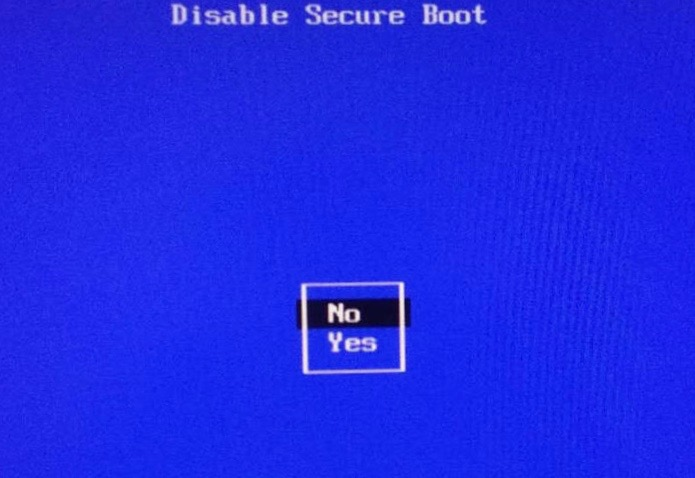
\includegraphics[width=0.7\textwidth]{mokutil}
\caption{صفحه\nf ای که پس از \lr{reboot} نمایش داده می\nf شود}
\label{mokutil}
\end{figure}

در این صفحه از شما پرسیده می\nf شود که آیا می\nf خواهید تنظیمات امنیّتی را تغییر دهید؟ گزینه \lr{Yes} را انتخاب کنید. پس از انتخاب این گزینه از شما خواسته می\nf شود که رمزعبوری را که ایجاد کرده\nf اید، وارد کنید. پس از وارد کردن رمز عبور، مراحل غیرفعّال کردن \lr{boot} امن پایان میابد. توجّه شود که در برخی از نسخه\nf های \lr{UEFI}، از شما نمی\nf خواهند که رمزعبور را به\nf طور کامل وارد کنید؛ بلکه می\nf خواهند بعضی از حروف رمزعبور را وارد کنید. مثلاً از شما می\nf خواهند که حرف اوّل، سوّم و هشتم رمزعبور خود را وارد کنید.
\begin{latin}
\setlength{\parindent}{0ex}
7. sudo apt-get install mokutil

8. sudo mokutil --disable-validation
\end{latin} 

\subsubsection{امضا کردن ماژول\nf ها}

برای امضا کردن ماژول\nf ها، ابتدا باید با دستور شماره\nf ی \lr{9}، کلیدهای لازم برای امضا کردن را ایجاد کرد. سپس، با اجرای دستور شماره\nf ی \lr{10}، ماژول\nf ها را امضا کرده و در آخر نیز با دستور شماره \lr{11}، کلیدها را در \lr{boot} امن، ثبت کرد. در صورتی که دستور شماره \lr{11} به\nf درستی اجرا نشد، ابتدا با دستور شماره \lr{7}، برنامه \lr{mokutil} را نصب کرده و سپس دستور شماره \lr{11} را اجرا کنید. پس از اجرای این دستور، از شما خواسته می\nf شود که یک رمزعبور به طول حدّاقل  8 حرف را ایجاد کنید. پس از انجام این کار، سیستم عامل را \lr{reboot} کنید. پس از انجام این مراحل، وارد صفحه\nf ای مشابه \ref{sign1} خواهیدشد.
\begin{latin}
\setlength{\parindent}{0ex}
9. openssl req -new -x509 -newkey rsa:2048 -keyout MOK.priv -outform DER -out MOK.der -nodes -days 36500 -subj "/CN=Descriptive name/"

10. sudo /usr/src/linux-headers-\$(uname -r)/scripts/sign-file sha256 ./MOK.priv ./MOK.der /path/to/module

11. sudo mokutil --import MOK.der
\end{latin}

\begin{figure}[H]
\centering
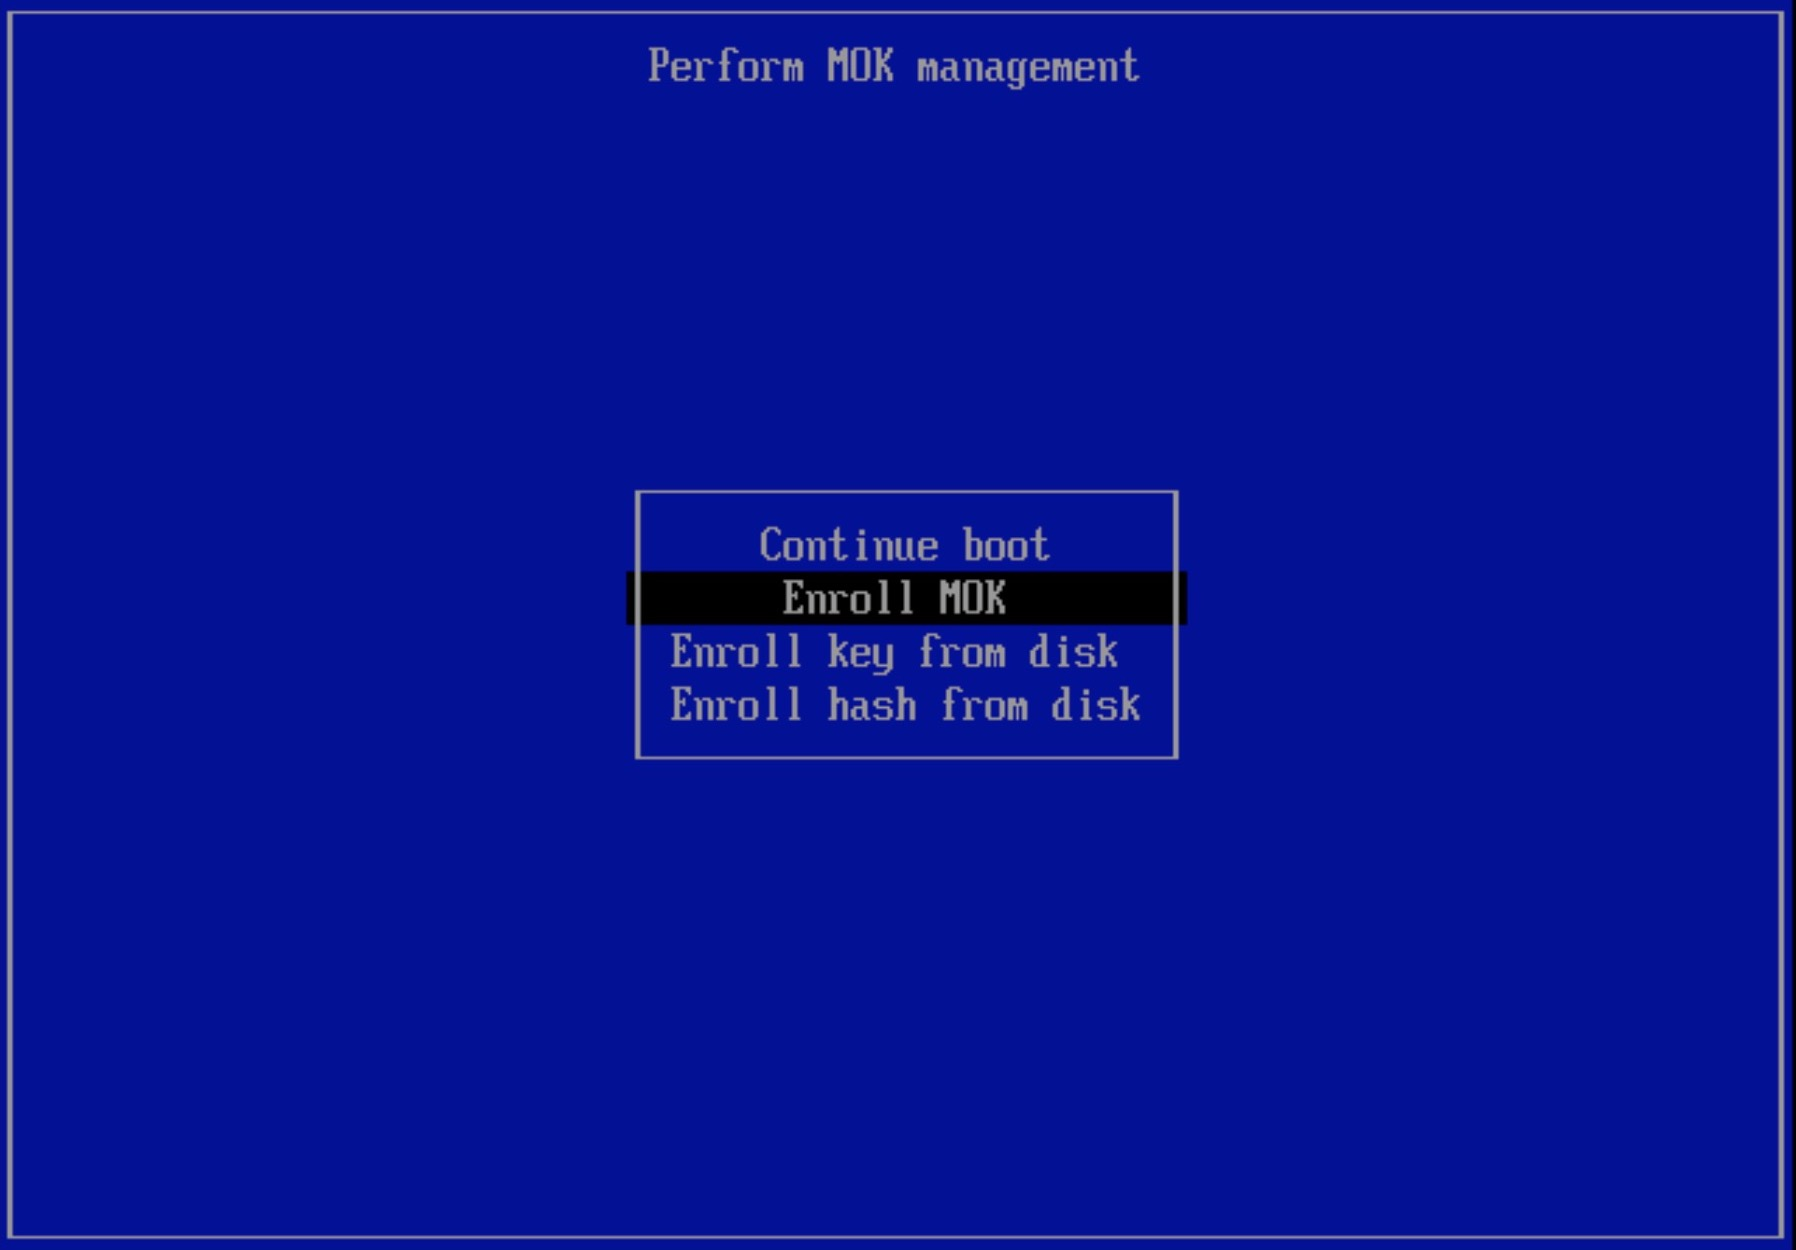
\includegraphics[width=.7\textwidth]{sign1}
\caption{مدیریت \lr{MOK}}
\label{sign1}
\end{figure}

در این صفحه، گزینه\nf ی \lr{Enroll MOK} را انتخاب کنید. سپس وارد صفحه\nf ای مشابه \ref{sign2} می\nf شوید. در این صفحه، گزینه \lr{Continue} را انتخاب کنید. سپس وارد صفحه\nf ی تأیید ثبت کلیدها(شکل \ref{sign3}) خواهیدشد. گزینه\nf ی \lr{Yes} را انتخاب کنید. مابقی مراحل، مانند روش قبل می\nf باشد؛ یعنی وارد صفحه\nf ای می\nf شوید که از شما خواسته می\nf شود رمزعبوری را که ساخته\nf اید وارد کنید.

\begin{figure}[H]
\centering
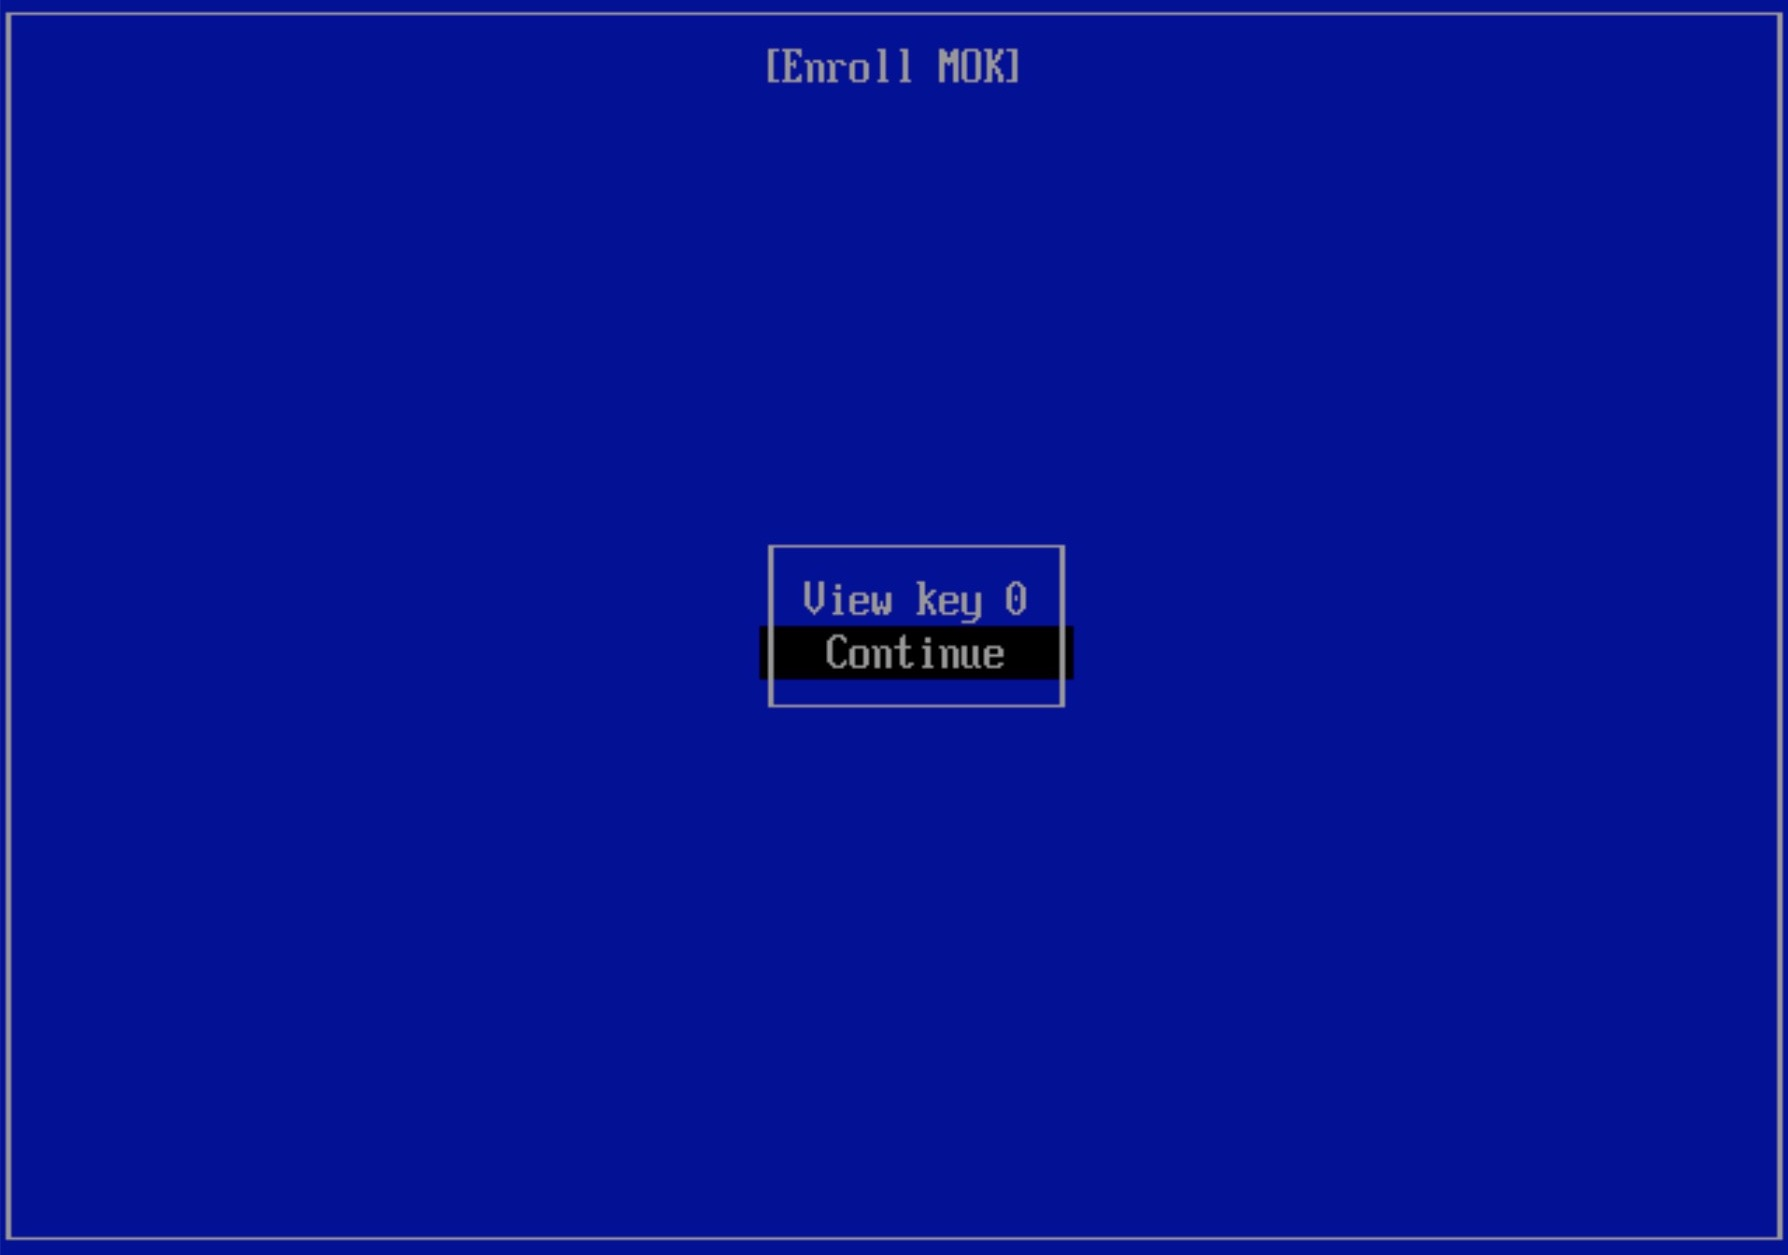
\includegraphics[width=0.7\textwidth]{sign2}
\caption{ثبت کلیدها}
\label{sign2}
\end{figure}


\begin{figure}[H]
\centering
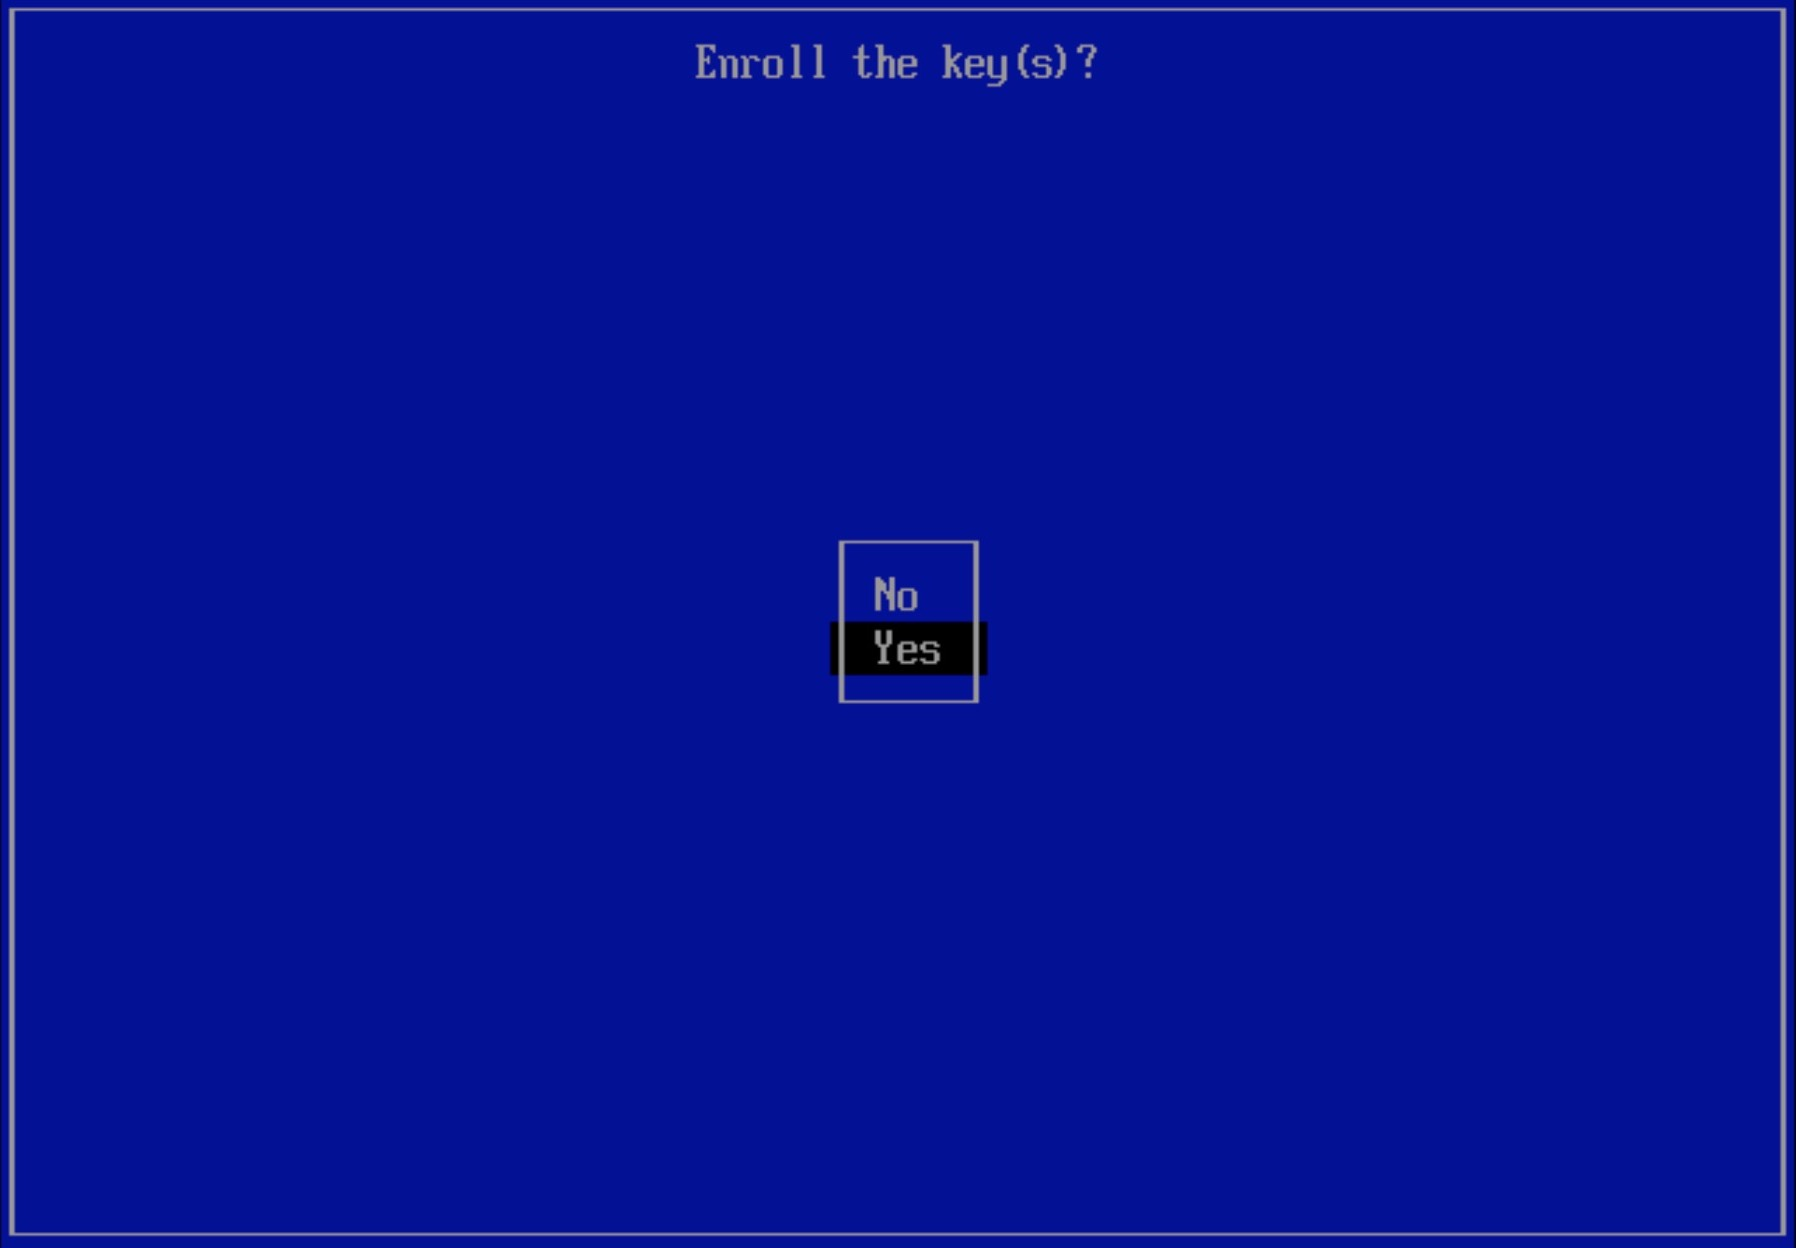
\includegraphics[width=0.7\textwidth]{sign3}
\caption{تأیید ثبت}
\label{sign3}
\end{figure}
